\documentclass[tikz,border=2pt]{standalone}
% shared tikz preamble for generating svg figures
% keep this file minimal; figure-specific styles can live in the figure .tex if needed
\usepackage{tikz}
\usetikzlibrary{positioning}
\usetikzlibrary{shapes.geometric}
\usetikzlibrary{arrows}
\usetikzlibrary{decorations}
\usetikzlibrary{decorations.markings}

\tikzset{>=latex}
\tikzstyle{Arrow} = [->, thin, preaction = {decorate}]
\tikzstyle{cor} = [-, dotted, preaction = {decorate}]

\begin{document}
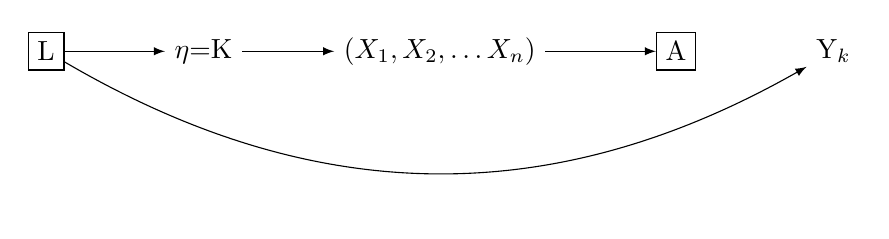
\begin{tikzpicture}[{every node/.append style}=draw]
\node [rectangle, draw=black] (L0) at (0, 0) {L};
\node [rectangle, draw=white] (K1) at (2, 0) {$\eta$=K};
\node [rectangle, draw=white] (X1) at (5, 0) {$(X_1, X_2, \dots X_n)$};
\node [rectangle, draw=black] (A1) at (8, 0) {A};
\node [rectangle, draw=white] (Y2) at (10, 0) {Y$_k$};

\draw [-latex, draw=black] (L0) to (K1);
\draw [-latex, bend right, draw=black] (L0) to (Y2);
\draw [-latex, draw=black] (K1) to (X1);
\draw [-latex, draw=black] (X1) to (A1);
\end{tikzpicture}
\end{document}
